\chapter{Background}

\section{Basic rules}
\label{sec:battling}
One of the key aspects of the Pokémon game is to battle other Pokémon. In the mainline games, you can 
have up to six Pokémon in your team, also known as party. There is the option to swap a Pokémon with
another Pokémon, but you can not have more than six Pokémon at any point in your team. When playing the 
original games, you explore the world to find more Pokémon and use your team to defeat wild Pokémon
and other Pokémon trainers. This thesis focuses on random battles taking place on Pokémon Showdown.
In a random battle, both competitors get a team of six random Pokémon. At the start of the battle,
you know each of your six Pokémon but only the currently active enemy Pokémon. \\
In every turn, both players can choose to either use a move of their currently active Pokémon or switch
their active Pokémon to another Pokémon. Moves can either deal direct damage to the enemy Pokémon or 
yield other advantages like increasing the damage dealt by the next move. Moves will be covered in more
detail in section \ref{sec:moves}. Each Pokémon has an amount of \ac{HP}. The \ac{HP} of a Pokémon
can be dropped by attacking it with a move. If the \ac{HP} of a Pokémon drops to zero, it faints and 
can not be used in this battle anymore. A player wins, once all enemies fainted. \\
Note that in the mainline games there is the possibility to heal or even revive a fainted 
Pokémon during battle using \textit{Healing Items} like \textit{Revive} or \textit{Hyper Potion}.
In competitive Play, only \textit{Held items} like \textit{Leftovers} are allowed. Items will be explained
in depth in section \ref{sec:items}.

\subsection{Types}
\label{sec:types}
Pokémon implements a \ac{RPS}-like system. Each Pokémon has either one or two of 
18 types. Like \emph{rock} beats \emph{scissors} but looses to \emph{paper}, \textit{Fire}-type Pokémon have an
\textit{advantage} against \textit{Grass}-type Pokémon but are on a \textit{disadvantage} against \textit{Water}-types.
This is also called a type being \textit{strong} / \textit{weak} against another type.
\begin{figure}
	\centering
	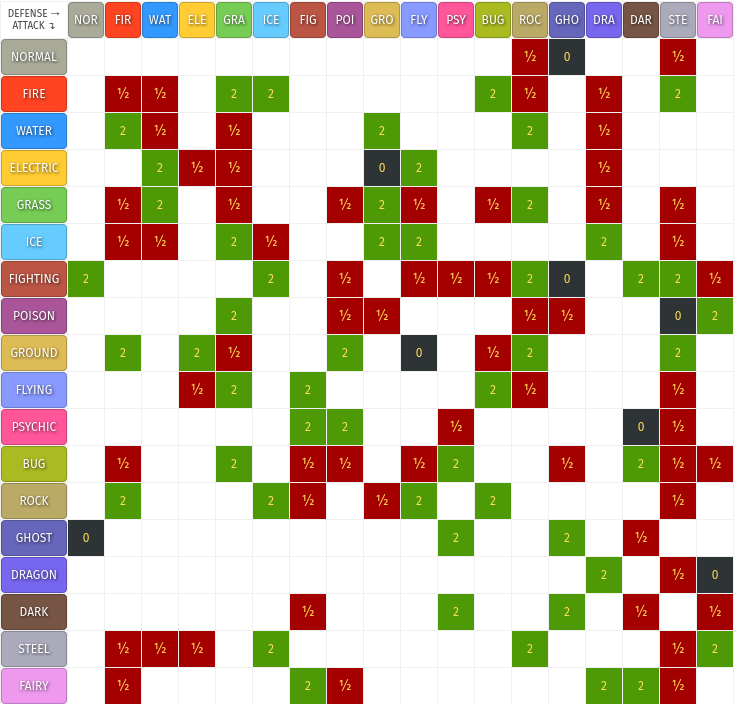
\includegraphics[width=0.7\textwidth]{images/type_chart.png}
	\caption{Advantages of different types ~\autocite{Pokemondb:Type}}
	\label{fig:type_chart}
\end{figure}
Figure \ref{fig:type_chart} shows how different Pokémon types interact with each other.
Unlike in \ac{RPS}, type modifiers will be multiplied if a Pokémon has two types. For instance, a \textit{Fire}-type
attack will deal 4 times the damage against \textit{Parasect} as \textit{Parasect} has the types \textit{Grass} and
\textit{Bug} ~\autocite{Veekun:Parasect}.

\subsection{Moves}
\label{sec:moves}
Moves can be split up into three categories: \textit{Physical}-, \textit{Special}- and \textit{Status}-Moves.
While \textit{Physical}- and \textit{Special}-Moves usually deal damage to the opponent Pokémon, 
\textit{Status}-Moves can for example change the weather, which plays a role in damage calculation explained
in section \ref{sec:damage-calculation}, inflict status effects, raise or lower the stats of a Pokémon. In 
addition, a move also has exactly one of the 18 possible types. Often, \textit{Status}-moves are also referred
to as \textit{buffing} moves if they grant a benefit to the user or as \textit{debuffing} if they have a
negative effect on the opponent.

\subsection{Pokémon}
\label{sec:pokemon}
A key-concept of Pokémon battles are the \textit{stats} of a Pokémon. 
\begin{figure}[h]
	\centering
	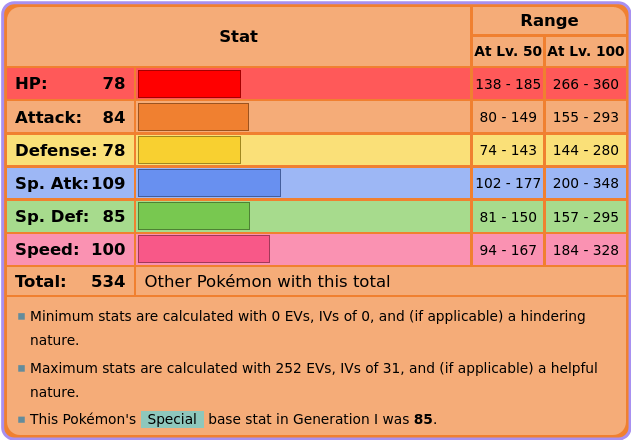
\includegraphics[width=0.7\textwidth]{images/charizard-stats.png}
	\caption{Possible stats of \textit{Charizard} ~\autocite{Bulbapedia:Charizard}}
	\label{fig:charizard-stats}
\end{figure}
Figure \ref{fig:charizard-stats} displays information about possible stat-combinations of 
\textit{Charizard}. 
\paragraph{Explanation of stats}
\textbf{HP:} The \ac{HP} determines how much damage a Pokémon can receive before fainting. \\
\textbf{Attack:} The \ac{ATK} determines how much damage a Pokémon will deal when using 
a \textit{Physical}-Move. \\
\textbf{Defense:} The \ac{DEF} determines how well a Pokémon can resist against \textit{physical} attacks. \\
\textbf{Sp. Atk:} The \ac{SPA} determines how much damage a Pokémon will deal when using
a \textit{Special}-Move. \\
\textbf{Sp. Def:} The \ac{SPD} determines how well a Pokémon can resist against special attacks. \\
\textbf{Speed:} The \ac{SPE} determines how fast a Pokémon can act. Usually, the Pokémon with a higher
\ac{SPE} will move before the slower one. The exact order of actions in battles is covered in section
\ref{sec:order-of-events}.
\todo{Cover evasion / accuracy, context to showdown}

\paragraph{Determination of stats}
\label{sec:stat-calculation}
The total stat of a Pokémon is calculated as described in equation \ref{eq:stats-hp} and equation 
\ref{eq:stats-other} ~\autocite{Bulbapedia:Stat}.
\begin{equation}
	\label{eq:stats-hp}
	HP = \Bigl\lfloor \frac{(2 \times Base + IV + \lfloor \frac{EV}{4} \rfloor) \times Level}{100}\Bigr\rfloor
	+ Level + 10 \\
\end{equation}
\begin{equation}
	\label{eq:stats-other}
	OtherStat = \Bigl\lfloor \Big( \frac{2 \times Base + IV + \lfloor \frac{EV}{4} \rfloor) \times Level}
	{100} + 5\Big) \times Nature \Bigr\rfloor
\end{equation}
\textbf{Base:} Refers to the base stat of a Pokémon. Two Pokémon of the same species will always have the 
same base-stats. As seen in figure \ref{fig:charizard-stats}, a \textit{Charizard} will always have a
base-\ac{ATK} of 84.

\textbf{Level:} As mentioned in section \ref{sec:battling}, the goal of the mainline games is to create 
a team of six Pokémon and to make that team stronger by fighting other Pokémon. If a Pokémon defeats
enough other Pokémon, it grows a Level. The maximum level of a Pokémon is 100.
In Pokémon Showdown, the level of  a Pokémon is set at the start of the battle and won't 
increase ~\autocite{Smogon:RandBatsGuide}.

\textbf{Nature:} A Pokémon has a nature. Most natures enhance the growth of one stat, while hindering
the growth of another. After all other calculations are finished, the stat that the Nature enhances will
be 100\% of what it would be without the Nature, and the stat hindered will be 90\% of its normal value
~\autocite{Bulbapedia:Stat}. In this thesis nature can be neglected as all Pokémon in random battles have
a neutral nature, meaning no stat is enhanced or hindered ~\autocite{Smogon:RandBatsGuide}.

\textbf{IV:} Refers to the \ac{IV} of a Pokémon. These cause two Pokémon of the same species to have
different Stats ~\autocite{Bulbapedia:Stat}. Pokémon in Pokémon Showdown will always have the best possible \ac{IV} 
stat, 31, unless it is a disadvantage for the Pokémon, then it will be zero ~\autocite{Smogon:RandBatsGuide}.
For example, having a high \ac{SPE} is undesirable for a Pokémon that uses the move \textit{Trick Room} as this
move reverses the move order so that Pokémon with a lower \ac{SPE} stat attack first while those with a 
higher \ac{SPE} will attack last.

\textbf{EV:} These are the \ac{EV} of the Pokémon. \ac{EV} are what causes a trained Pokémon to have higher
stats than an untrained counterpart of the same level. For every 4 \ac{EV} gained, a level 100 Pokémon 
will have 1 extra point in the given stat. A Pokémon can earn up to 510 \ac{EV}, but can not have more than
255 \ac{EV} in a single stat ~\autocite{Bulbapedia:Stat}. Random Pokémon on Showdown will always have 85 
\ac{EV} in each stat, or 0 in the case that having a high stat being detrimental ~\autocite{Smogon:RandBatsGuide}.

\subsection{Switching}
\label{sec:switching}
Instead of using a move with the current Pokémon, the player also has the option to switch out the 
active Pokémon for another Pokémon is his party. Switching always takes place before the execution of moves.
However, the player does not know whether the opponent is switching or using a Move. Therefore, if the 
player decides to switch out a non-fainted Pokémon, the enemy gets to use his move on the new Pokémon.
If a Pokémon faints, the player has to switch in a new Pokémon and then the next turns tarts. This means
that the opponent gains a one turn advantage if the player decides to switch out a healthy Pokémon, but
won't get to attack an additional time if the Pokémon was defeated.  

\subsection{Status condition}
Moves may inflict so-called \textit{status conditions} that affect a Pokémon negatively.
The most important status conditions are
\begin{itemize}
	\item \textbf{Burn:} If a Pokémon suffers from the status condition \ac{BRN}, it will lose 1/8 of its
		total \ac{HP} every turn. In addition to that, a burned Pokémon will only deal half as much damage
		when using a \textit{physical} move.
	\item \textbf{Freeze:} If a Pokémon suffers from the status condition \ac{FRZ} it won't, with a few exceptions,
		be able to use moves. 
	\item \textbf{Paralysis:} If a Pokémon suffers from the status condition \ac{PAR} it won't be able to use 
		the selected move 25\% of the time and their speed is halved.
	\item \textbf{Poison:} If a Pokémon suffers from the status condition \ac{PSN} it will, with a few exceptions,
		take damage equal to 1/8 of its total \ac{HP} at the end of every turn. A Pokémon can also be 
		\textit{badly poisoned}. Badly poison initially inflicts damage equal to 1/16 of the Pokémon's maximum
		\ac{HP}, with the damage inflicted increasing by 1/16 each turn. This means that the Pokémon will
		take 2/16 damage on the second turn, 3/16 on the third turn (and so on).
	\item \textbf{Sleep:} If a Pokémon suffers from the status condition \ac{SLP} it won't be able to use moves,
		except \textit{Snore} and \textit{Sleep Talk}. In the mainline games, sleep lasts randomly between
		one and three turns. However, in Pokémon Showdown a Pokémon will \textit{always} be asleep for exactly
		two turns.
\end{itemize}

At any point, a Pokémon can only suffer from one status condition at a time, this means that a 
burned Pokémon can not fall asleep. While a sleeping Pokémon wakes up after a few turns and a 
frozen Pokémon is unfrozen after a few turns, the other status conditions remain until they are 
cured. A status condition can either be cured by abilities like \textit{Natural Cure}. This ability
heals any status condition when the Pokémon is switched out. Items can also remove negative effects,
for example, \textit{Lum Berry} cures all status conditions but gets consumed in the process.
\todo{How long are Pokémon asleep / frozen?}

\subsection{Items}
\label{sec:items}
A Pokémon can also hold an Item that yields benefits in battle. There are various purposes that items 
can fulfill. For example, the item \textit{Life Orb} boosts damage dealt by the holder's damaging move
by 30\%\footnote{This boost is approximated as 5324/4096 $\approx$ 1.29980}, but the holder takes
damage equal to 10\% of its maximum \ac{HP} after it uses a damaging move\footnote{Rounded down, 
but not less than 1} ~\autocite{Bulbapedia:LifeOrb}. \textit{Leftovers} restore 1/16 of the holder's
maximum \ac{HP}\footnote{Rounded down, but not less than 1} at the end of each turn whereas the item
\textit{Air Balloon} makes the holder \textit{ungrounded}, which means that the holder is immune to
\textit{Ground}-type moves as well as several related effects~\autocite{Bulbapedia:AirBalloon}. The 
generation of items in Pokémon Showdown is described in more detail in section \ref{sec:randbats-items}.
\paragraph{Important items}
\label{sec:Important-items}
In this section, a quick introduction to the most important items is given.
\begin{itemize}
	\item \textbf{Choice Band:} When held by a Pokémon, this item boosts the \ac{ATK} by 50\%, but only
	allows the use of the first move selected. This effect resets when the holder is switched out ~\autocite{Bulbapedia:ChoiceBand}. 
	\item \textbf{Choice Scarf:} When held by a Pokémon, this item boosts the \ac{SPE} by 50\%, but only
	allows the use of the first move selected. This effect resets when the holder is switched out ~\autocite{Bulbapedia:ChoiceScarf}. 
	\item \textbf{Choice Specs:} When held by a Pokémon, this item boosts the \ac{SPA} by 50\%, but only
	allows the use of the first move selected. This effect resets when the holder is switched out ~\autocite{Bulbapedia:ChoiceSpecs}. 
	\item \textbf{Heavy-Duty Boots:} The holder is unaffected by the effects of entry hazards. Entry hazards are described 
	in \ref{sec:hazards}.
	\item \textbf{Assault Vest:} Raises the holders \ac{SPD} by 50\% but also prevents the holder from selecting any 
	status move\footnote{Except \textit{Me First}} ~\autocite{Bulbapedia:AssaultVest}.
	\item \textbf{Focus Sash:} If the holder has full \ac{HP} and is hit by an attack that would otherwise cause fainting,
	it survives with 1 \ac{HP} ~\autocite{Bulbapedia:FocusSash}.
\end{itemize}

\subsection{Field effects}
\label{sec:field-effects}
There are multiple \textit{field effects} that affect combat. Field effect are different from items as they are not
tied to a specific Pokémon but rather always effect the currently battling Pokémon. There are field effects that only
target the side of one player as well as effects that target both sides. 
\paragraph{Terrain}
\textit{Terrain} is set up by the respective move with identical name and last for five turns and effects both players.
All of them are beneficial to \textit{grounded} Pokémon. A Pokémon is \textit{not grounded} if any of the 
following conditions apply: The Pokémon
\begin{itemize}
	\item has the \textit{Flying}-type
	\item has the Ability \textit{Levitate}
	\item is holding the item \textit{Air Balloon}
	\item is under the effect of \textit{Magnet Rise} or \textit{Telekinesis}.
\end{itemize}
\textit{Grounded} Pokémon are with a few exceptions those Pokémon, that are not \textit{ungrounded}. A 
Pokémon will be grounded if any of the following conditions apply:
\begin{itemize}
	\item The Pokémon is holding an \textit{Iron Ball}
	\item The Pokémon is under the effect of \textit{Ingrain}, \textit{Smack Down} or \textit{Thousand Arrows}.
	\item The \textit{Field effect} \textit{Gravity} is in effect.
\end{itemize}
More information about grounding can be found at ~\autocite{Bulbapedia:Grounded}
There are five different possible \textit{terrain}-states. 
\begin{itemize}
	\item \textbf{None:} The default state, no other effects are applied. 
	\item \textbf{Electric Terrain:} Grounded Pokémon can not fall asleep and the power of \textit{Electric}-type
		moves is increased by 50\%.
	\item \textbf{Grassy Terrain:} The HP of grounded Pokémon is restored by 1/16 of their maximum HP at the
		end of each turn. In addition, the power of \textit{Grass}-type moves is increased by 50\% and the 
		moves \textit{Earthquake}, \textit{Magnitude} and \textit{Bulldoze} halve in power. 
	\item \textbf{Misty Terrain:} Protects all grounded Pokémon from status conditions (including confusion)
		\todo{Does confusion exist in Showdown?}
		The power of \textit{Dragon}-type moves is halved while in effect. 
	\item \textbf{Psychic Terrain:} Prevents grounded Pokémon from being hit by priority moves. Priority
	moves will be covered in section \ref{sec:order-of-events}. The power of \textit{Psychic}-type moves is also increased
\end{itemize}
It is important to note that only one \textit{terrain} can be active at a time, yet, \textit{terrain}
can coexist with other \textit{field effects} like \textit{weather}.

\paragraph{Weather}
The \textit{weather} is a set of mechanics that change the battle environment, activating abilities, modifying
certain moves and potentially damaging the Pokémon in battle or affecting their stats. Only one type of weather may 
be present at a time, and only the most recent type of weather will take effect \cite{Bulbapedia:Weather}. List
of different \textit{weather}-conditions:
\begin{itemize}
	\item \textit{Clear skies}: (also: \emph{None}) Absence of weather, this is the default state
	\item \textit{(Harsh-) Sunshine:} (also: \emph{(Harsh-) Sunlight}) Strong sunlight shines on the 
	battlefield
	\item \textit{(Heavy-) Rain:} Rain falls on the battlefield.
	\item \textit{Sandstorm:} Stinging sand whips across the battlefield. At the end of each turn, each
	Pokémon, with a few exceptions, takes damage equal to $1/16$ of its maximum \ac{HP} unless it is 
	a \textit{Rock}-, \textit{Steel}- or
	\textit{Ground}-type. \todo{https://bulbapedia.bulbagarden.net/wiki/Sandstorm_(weather_condition)}
	\item \textit{Hail:} Pelting hail falls on the battlefield. At the end of each turn, each
	Pokémon, with a few exceptions, takes damage equal to $1/16$ of its maximum \ac{HP} unless it is an \textit{Ice}-type.
	\todo{https://bulbapedia.bulbagarden.net/wiki/Hail_(weather_condition)}
\end{itemize}
There are a few additional special weather conditions which will not be covered in this thesis as they only occur in 
very specific scenarios.

\paragraph{Other}
The list below contains the remaining field effects that cover the entire field not covered so far:
\begin{itemize}
	\item \textit{Wonder Room:} swaps the \ac{DEF} and \ac{SPD} of all Pokémon, but stat changes
	remain on their respective stat. \todo{https://bulbapedia.bulbagarden.net/wiki/Wonder_Room_(move)}
	\item \textit{Magic Room:} suppresses the effect of all items held by the Pokémon on the field
	\todo{https://bulbapedia.bulbagarden.net/wiki/Magic_Room_(move)}
	\item \textit{Gravity:} causes the field to undergo intense gravity which multiplies the accuracy stat of
	all Pokémon by $5/3$ \todo{https://bulbapedia.bulbagarden.net/wiki/Gravity_(move)}
	\item \textit{Trick Room:} reverses the move order within each priority bracket. Move priority will be covered
	in section \ref{sec:order-of-events}
\end{itemize}
\todo{According to Bulbapedia: All last for 5 turns}

\paragraph{Single Side Effects}
Among \textit{Hazards} which will be covered in section \ref{sec:hazards}, the most important single side
effects are \textit{Reflect} which halves the damage done to Pokémon on the given side by \textit{physical}
moves \todo{https://bulbapedia.bulbagarden.net/wiki/Reflect_(move)} and \textit{Light Screen} which works
equivalent but for \textit{special} moves \todo{https://bulbapedia.bulbagarden.net/wiki/Light_Screen_(move)}

\subsection{Order of events}
\label{sec:order-of-events}
In battle, switching always is executed before moves meaning that if a player switches and his opponent chooses
to use a move, the move will always hit the newly brought in Pokémon. Move order is determined based on
\textit{priority}.
\paragraph{Priority}
\textit{Priority} is a characteristic of moves, such that any move with a higher priority will always be
performed first. When two moves have the same priority, the users \ac{SPE} stat will determine which
one is performed first in battle. Each move has a hidden priority value in the game data, with values ranging
from $+5$ to $-7$ The vast majority of moves have the standard priority value of 0. A move with a positive
priority is called \textit{priority move}. Moves that have the same priority are said to be in the same
priority bracket. An example for a move with priority $+2$ is \textit{Extreme Speed}, a \textit{Normal}-type
move with a base-power of $80$\todo{https://bulbapedia.bulbagarden.net/wiki/Extreme_Speed_(move)}. Having
a \textit{priority}-move can be useful if the own active Pokémon has a lower \ac{SPE}-stat than the 
opponent with low \ac{HP} as then the own Pokémon does not have to take an additional hit before defeating
his enemy. 

\subsection{Damage calculation}
\label{sec:damage-calculation}
The damage dealt by a move mainly depends on the \textit{level} of the Pokémon
that uses the move, its effective Attack or Special Attack stat, the
opponent's effective Defense or Special Defense stat and the move's effective
power. 

Precisely, the damage is calculated as follows~\autocite{Bulbapedia:Damage}:
\begin{dmath}
  \text{Damage} = \left(\frac{\left(\frac{2 \times \text{Level}}{5}\right) \times \text{Power} \times \text{A / D}}{50} + 2\right)
	\times Targets
	\times Weather
	\times Badge
	\times Critical
	\times random
	\times STAB
	\times Type
	\times Burn
	\times other
\end{dmath}

The only exception for this are moves that deal direct damage. A list 
of these moves can be found at ~\autocite{Bulbapedia:DirectDamage}.
In the following paragraph, parameters of the formula are covered in detail. An
explanation of the \textit{Type}-modifier is omitted since it is covered in 
\ref{sec:types}

\paragraph{Level}
\textit{Level} refers to the level of the attacking Pokémon~\autocite{Bulbapedia:Damage}. 
In Pokémon Showdown, the level is displayed next to the name of the Pokémon.

\paragraph{A / D}
\textit{A} is the effective Attack stat of the attacking Pokémon if the used move is a physical move,
or the effective Special Attack stat of the attacking Pokémon if the used move is a special move.
\\
\textit{D} is likewise the effective Defense stat of the target if the used move is a physical move,
or the effective Special Defense of the target if the used move is a special move~\autocite{Bulbapedia:Damage}.

There are four moves that use stats from different categories, more Information can be found
at ~\autocite{Bulbapedia:MoveStatDifferentCategories}.

\paragraph{Power}
Power is the effective power of the used move.
The \textit{Base Power} of a move in Showdown can be seen when hovering over a move in the move list. \\
\textit{Note:} The same move will always have the same base power. For example, \textit{Fire Punch} will
always have a base power of 75~\autocite{Bulbapedia:FirePunch}.

\paragraph{Weather}
The \textit{Weather} modifier is 1.5 if a \textit{Water-type} move is used during \textit{rain} or a 
\textit{Fire-type} move during \textit{Harsh Sunlight}. The modifier is 0.5 if a \textit{Water-type} move
is used during \textit{Harsh Sunlight} or a \textit{Fire-type} move during \textit{rain} ~\autocite{Bulbapedia:Damage}.

\paragraph{Critical}
In the latest generation, a \ac{CRIT} deals 1.5 times the damage compared to a normal hit.
If the \ac{CRIT} rate is not increased, the chance of landing a \ac{CRIT} is 1/24
~\autocite{Bulbapedia:CriticalHit}. Increasing \ac{CRIT} rate, as well as other stats, will 
be explained in chapter \ref{sec:boosting}. \\
\textit{Note:} In earlier games, \ac{CRIT}s worked different, see ~\autocite{Bulbapedia:CriticalHit} for
more details.

\paragraph{Random}
\textit{Random} is a random integer percentage between 85\% and 100\%. Because of this, the same move
may deal different damage in the same scenario ~\autocite{Bulbapedia:Damage}.

\paragraph{STAB}
\textit{STAB} stands for \textit{Same Type Attack Bonus}. It is a multiplier of 1.5 if the current move
is of the same type as the attacking Pokémon. Otherwise, it is 1.0 ~\autocite{Bulbapedia:Damage}.

\paragraph{Type}
This is the in type modifier described in section \ref{sec:types}~\autocite{Bulbapedia:Damage}.

\paragraph{Burn}
\textit{Burn} is 0.5 if the attacking Pokémon is burned, and the attack
is physical\footnote{This does not apply if the attacking Pokémon has the Ability \textit{Guts}
or the used move is \textit{Facade}}. Otherwise, it is 1.0 ~\autocite{Bulbapedia:Damage}.

\paragraph{Other}
The \textit{other} modifier is usually 1. A list of exceptions can be found at ~\autocite{Bulbapedia:Damage}.

\subsection{Effective Stats}
\label{sec:boosting}
When a stat is used in a calculation in battle, a number of modifiers may be applied during the calculation.
During a battle, a Pokémon's effective stats may be raised or lowered by certain moves abilities and 
held items. Some attacks may only have a chance of lowering stats, while certain abilities and held items
may require a triggering event to activate stat modifications. \\
The modifiers conferred by most moves operate on a sliding scale of \textit{stages}. When a given stat is raised
or lowered, its current stage is increased or decreased by the amount dictated by the move; Up to a maximum
of $+6$ or a minimum of $-6$. A given stat corresponds to a given multiplier that will modify the stat when it
is used in calculations. The exact multipliers for stages are described in table \ref{tab:boost-stage-multipliers}
\begin{table}[h]
	\centering
	\begin{tabular}{|c|c|c|c|c|c|c|c|c|c|c|c|c|c|}
		\hline
		-6 & -5 & -4 & -3 & -2 & 1 & 0 & 1 & 2 & 3 & 4 & 5 & 6 \\
		\hline
		$2/8$ & $2/7$ & $2/6$ & $2/5$ & $2/4$ & $2/3$ & $2/2$ &  $3/2$ &  $4/2$ &  $5/2$ &  $6/2$ &  $7/2$ & $8/2$ \\
		\hline
	\end{tabular} 
	\caption{Stage multipliers for \ac{ATK}, \ac{DEF}, \ac{SPA}, \ac{SPD} and \ac{SPE}}
	\label{tab:boost-stage-multipliers}
\end{table}
\todo{Table / Text source:https://bulbapedia.bulbagarden.net/wiki/Stat\#Stat_modifiers}
\todo{Other table for accuracy an evasion}
When playing the mainline games, the player has to memorize the current stat changes of a Pokémon. In contrast to that,
Pokémon Showdown displays the current stat multiplier of both Pokémon. Stat changes caused by boosts do not persist
between switches, meaning that the stages for all stats of a Pokémon are reset to zero upon being switched in.

\section{Dynamaxing}
Dynamaxing is a temporary transformation affecting Pokémon that was introduced in Generation eight. Dynamaxing increases
a Pokémon's size drastically, as well as changing the moves of the Pokémon and doubling their max and current \ac{HP},
but can only be used once per battle and ends after three turns or if the Pokémon is switched out.

\section{Hazards}
\label{sec:hazards}
An \textit{entry hazard} is a condition that affects one side of the field. It causes
any Pokémon that is sent into battle on that side of the field to be afflicted by 
a negative effect. Entry hazards are created by moves, usually status moves
~\autocite{Bulbapedia:EntryHazards}. \\
\subsection{List of entry hazards}
Currently, there are five moves that create an entry hazard

\paragraph{Spikes}
\textit{Spikes} is a \textit{Ground}-type entry hazard that causes the opponent
to lose $1/8$\% of their maximum \ac{HP} when they enter the field. This
effect can be stacked up to three times. Two layers of spikes will deal
$1/6$\% and three layers will deal $1/4$\% of the enemies maximum \ac{HP}.
Spikes are set by the move \textit{Spikes}~\autocite{Bulbapedia:Spikes}.

\paragraph{Stealth Rock}
\label{sec:stealthrock}
The move \textit{Stealth Rock} sets an entry hazard around the target Pokémon
causing Pokémon on the target's field to receive damage upon being switched in.
The amount of damage inflicted is affected by the effectiveness of the type
\textit{Rock} against the target. Unlike Spikes, this entry hazard does not stack.
The damage taken from the victim's maximum is denoted in table 
\ref{tab:stealth-rock-damage}~\autocite{Bulbapedia:StealthRock}.
\begin{table}[h]
	\centering
	\begin{tabular}{|c|c|}
		\hline
		\textbf{Type effectiveness} & \textbf{Damage (Max. \ac{HP}}) \\
		\hline 
		0.25x & 3.125\% \\ 
		\hline 
		0.5x &  6.25\% \\ 
		\hline 
		1x & 12.5\% \\
		\hline
		2x & 25\% \\
		\hline
		4x & 50\% \\
		\hline
	\end{tabular} 
	\caption{Damage dealt to Pokémon by Stealth Rocks~\autocite{Bulbapedia:StealthRock}}
	\label{tab:stealth-rock-damage}
\end{table}

\paragraph{Sticky Web}
The entry hazard set by the \textit{Bug}-type move \textit{Sticky Web} lowers the
opponents speed stat by one stage upon switching in ~\autocite{Bulbapedia:StickyWeb}. \\
\todo{Pokémon that are not affected by this}

\paragraph{Poison spikes}
\label{sec:poison-spikes}
\textit{Poison Spikes} set by the \textit{Poison}-type move \textit{Toxic Spikes}
cause the opponent to become poisoned. If two layers of spikes are set, the
Pokémon instead becomes badly poisoned ~\autocite{Bulbapedia:ToxicSpikes}. \\
\todo{Pokémon not affected} \\

\paragraph{Sharp steel}
This entry hazard works very similar to Stealth Rock described in \ref{sec:stealthrock}.
However, Sharp steel can only be set by the \textit{Steel}-type move
\textit{G-Max Steelsurge} which is the exclusive G-Max Move of \textit{Gigantamax Copperhead}
\todo{Add source}.
The damage dealt by Sharp steel does not stack, the amount of damage dealt is
based on the Type effectiveness of the \textit{Steel}-type against the target.
Exact damage modifiers can be found in table \ref{tab:sharp-steel-damage}
~\autocite{Bulbapedia:GMaxSteelsurge}.
\begin{table}[h]
	\centering
	\begin{tabular}{|c|c|}
		\hline
		\textbf{Type effectiveness} & \textbf{Damage (Max. \ac{HP}}) \\
		\hline 
		0.25x & 3.125\% \\ 
		\hline 
		0.5x &  6.25\% \\ 
		\hline 
		1x & 12.5\% \\
		\hline
		2x & 25\% \\
		\hline
		4x & 50\% \\
		\hline
	\end{tabular} 
	\caption{Damage dealt to Pokémon by Sharp Steel~\autocite{Bulbapedia:GMaxSteelsurge}}
	\label{tab:sharp-steel-damage}
\end{table}

\subsection{Hazard counterplay}
There are some moves that can remove entry hazards. \textit{Rapid Spin} 
~\autocite{Bulbapedia:RapidSpin} removes entry hazards from the user's side of the field and
\textit{Defog}~\autocite{Bulbapedia:Defog} removes entry hazards on both sides of the 
field\footnote{In older games \textit{Defog} would only remove Hazards on the
target's side of the field. But as we only investigate the latest version, this
won't be covered in detail.}. In addition, 
\textit{Court Change}~\autocite{Bulbapedia:CourtChange} will exchange the entry hazards
on each side of the field, along with other one-sided field conditions.
If a grounded\footnote{The term \textit{grounded} is used to describe a Pokémon that
can not be affected by damaging \textit{Ground}-type moves and several other associated 
effects~\autocite{Bulbapedia:Grounded}.}
\textit{Poison}-type Pokémon enters the battle, it will remove Toxic 
Spikes, described in \ref{sec:poison-spikes}, from its side of the field.
Pokémon holding the item 
\textit{Heavy-Duty Boots}~\autocite{Bulbapedia:HeavyDutyBoots} are unaffected by
entry hazards, but grounded \textit{Poison}-type Pokémon can still remove
Toxic Spikes even if they hold the boots~\autocite{Bulbapedia:EntryHazards}.
Additionally, there are various other exceptions to hazards which won't be covered in detail here.

\section{Showdown random battles}
Pokémon Showdown features a large variety of game modes, the most popular ones being \textit{Sw / Sh Singles OU} and
\textit{Sw / Sh Singles Random Battle}. \textit{Sw / Sh} refers to Pokémon \textit{Sword} and \textit{Shield}, the latest
Pokémon Games. These two games form the eight generation of Pokémon games and are thereby also often referred as 
\textit{Gen8}-games. As Pokémon Showdown solely focuses
on battling every player has access to every available Pokémon. This mainly plays a role in the \textit{OU}-format.
In this game mode, each player knows all enemy Pokémon but does not know their exact builds, that is, the abilities,
\ac{IV}-, \ac{EV}-combinations and items are unknown. As the success of a player in this format heavily depends
on his team as well as which other teams are currently popular, this thesis will focus on random battles. In this 
format, each player gets a team of six random Pokémon and unlike in \textit{OU} only knows the currently active
opposing Pokémon. It is important to note that there are many possible builds for a Pokémon and therefore, information
management plays a huge role. An example for this will be provided in section \ref{sec:builds-randbats}. \\
The development for battling bots is explicitly allowed and encouraged by the developers. Furthermore, there is 
no way to figure out whether the current opponent is a real human or an AI. This is beneficial as humans
might behave differently when they know they are facing a machine potentially leading to invalid results. 

\label{sec:showdown-randbats}
\subsection{Sets}
\label{sec:randbats-sets}
As described in section \ref{sec:stat-calculation}, Pokémon created for random battles
usually have 85 \ac{EV}s and 31 \ac{IV} in every stat with a neutral nature, 
meaning a nature that does neither boost nor hinder any stat ~\autocite{Smogon:RandBatsGuide}.
There are some cases where a high stat is not beneficial, an example would be the 
move \textit{Gyro Ball}. Unlike most moves, the \textit{Base Power} of this move
described in the damage calculation described in \ref{sec:damage-calculation} is not
a fixed value. It is determined as described in \ref{eq:gyroball-base-power} ~\autocite{Bulbapedia:GyroBall}.
\begin{equation}
	\label{eq:gyroball-base-power}
	BasePower = \min\left( 150, \frac{25 \times CurrentSpeed_{target}}{CurrentSpeed_{user}}\right)
\end{equation} 
Since the damage dealt by \textit{Gyro Ball} gets bigger, the lower the \ac{SPE} of the
attacker, Pokémon using this move have 0 \ac{EV} and 0 \ac{IV} in the \ac{SPE} stat. \\
\textit{Note:} Being able to outspeed the opponent is extremely valuable, but the only
two Pokémon using \textit{Gyro Ball}, \textit{Stakataka} and \textit{Ferrothron}, already
have a very low \ac{SPE} stat and are slower than almost all other Pokémon in random
battles. A complete list of Pokémon with their respective \ac{SPE} stat can be found
at ~\autocite{Bulbapedia:PokemonBySpeed}. \\
This knowledge can be exploited to gather additional information about the enemy. Section
\ref{sec:builds-randbats} describes how this is achieved.

\subsection{Items}
\label{sec:randbats-items}
Items in random battles are procedurally generated by showdown and depend on the Pokémon's
moves, base stats and ability. As stated in ~\autocite{Smogon:RandBatsGuide}, the exact implementation
is \grqq changed frequently with the intention of optimizing set generation\grqq, yet, item
assignment follows these rules:
\begin{itemize}
	\item Pokémon with 2 or fewer attacking moves will get \textit{Leftovers}, or 
	\textit{Black Sludge} if \textit{Poison}-type.
	\item Pokémon with 3 attacking moves will get \textbf{Life Orb}, if the sum of their base
	\ac{HP}, \ac{DEF} and \ac{SPD} is less than 275. Otherwise, these Pokémon get 
	\textit{Leftovers} or \textit{Black Sludge}.
	\item Pokémon with 4 matching attacks get a \textit{Choice} item which follows these rules:
	\begin{itemize}
		\item Pokémon with four physical attacks or four special attacks, a base \ac{SPE} between
		60 and 108 and base \ac{ATK} or \ac{SPA} of 100 or more can get a \textit{Choice Scarf}
		2/3 of the time. If the Pokémon does not meet one of the stat qualifications or does not
		get the 2/3 chance, they'll get \textit{Choice Specs} or \textit{Choice Band} instead.
		\item Pokémon with 3 special attacks and the move \textit{U-turn} always get 
		\textit{Choice Specs}. \textit{U-turn} is a physical, \textit{Bug}-type move that 
		switches the user out after damage is dealt ~\autocite{Bulbapedia:UTurn}.
		\item Pokémon with \textit{Trick} ~\autocite{Bulbapedia:Trick} or \textit{Switcheroo} 
		~\autocite{Bulbapedia:Switcheroo}, both moves that allow to switch items
		with the opponent, will always get a choice item. If they meet the above-mentioned 
		speed range, they will always get a \textit{Choice Scarf}. Otherwise, they will always
		get \textit{Choice Specs} or \textit{Choice Band}.
		\item Having priority moves will always prevent a \textit{Choice Scarf} from being 
		generated in all situations.
	\end{itemize}
	\item Pokémon with 4 attacks that do not qualify for choice items, will get an \textit{Assault
	Vest} if their \ac{HP} + \ac{DEF} + \ac{SPD} $\geq$ 235. Otherwise, \textit{Expert Belt},
	\textit{Leftovers} or \textit{Life Orb} is generated.
	\item Pokémon that are weak to Rock will get \textit{Heavy-Duty Boots} if they don't get a 
	higher priority item, such as \textit{Assault Vest} or a choice item. Pokémon that are four
	times weak to \textit{Rock}, such as \textit{Charizard}, will always get \textit{Hevay-Duty Boots}.
	This is done as these Pokémon would otherwise lose up to 50\% \ac{HP} to the entry hazard
	\textit{Stealth Rock} described in \ref{sec:stealthrock}. The only exception is \textit{Scyther},
	which can get \textit{Eviolite}.
	\item Pokémon in the lead slot will get \textit{Focus Sash} if their \ac{HP} + \ac{DEF} + \ac{SPD} < 255,
	and they would otherwise get \textit{Leftovers} or \textit{Life Orb}.
	\item Pokémon that get a Speed-boosting move will be given a \textit{Weakness Policy} if their \ac{HP}
	+ \ac{DEF} + \ac{SPD} $\geq$ 300, and they aren't four times weak to \textit{Ground}. This item
	boosts the \ac{ATK} and \ac{SPA} by two stages each if hit by a super effective move. After that,
	the item breaks ~\autocite{Bulbapedia:WeaknessPolicy}.
\end{itemize}
There are also some species that will always roll the same item, either because it's their signature item or
because doing so supports a niche ability or set. For example, Pikachu always has \textit{Light Ball}

\section{Pokémon Matchups}
Due to the typing system, there is no best Pokémon that is the best option in all situations. Therefore, we 
have to determine how good a Pokémon is against another Pokémon in a given situation. In this case, the
\textit{situation} refers to the current state of both Pokémon like current \ac{HP} and status conditions
as well as field effects like weather. 
\subsection{Check and Counter}
There are multiple definitions of \textit{check} and \textit{counter} \todo{Cite multiple definitions}. In
this thesis, we refer to a Pokémon \textit{checking} another Pokémon if it can beat the enemy Pokémon in 
every scenario and can safely be switched in at any point. A \textit{counter} is also capable of defeating
the enemy Pokémon but may lose in some situations. The most notable being if switched in without the
previous active Pokémon fainting as this grants the opponent an additional attack. \\
The key difference between \textit{check} and \textit{counter} is that a check is also stronger if
it takes damage once more while a counter is not guaranteed to win in this situation. \\
\textit{Note:} Every \textit{check} to a Pokémon is also always a \textit{counter} while \textit{counter}
could also be a \textit{check}, but is not guaranteed to. 